\documentclass[aspectratio=169]{beamer}
%
% Choose how your presentation looks.
%
% For more themes, color themes and font themes, see:
% http://deic.uab.es/~iblanes/beamer_gallery/index_by_theme.html
%
\mode<presentation>
{
  \usetheme{metropolis}      % or try Darmstadt, Madrid, Warsaw, ...
  \usecolortheme{metropolis-imagelab} % or try albatross, beaver, crane, ...
  \usefonttheme{structurebold}  % or try serif, structurebold, ...
  \setbeamercolor{background canvas}{bg=white}
  \setbeamertemplate{navigation symbols}{}
  \setbeamertemplate{bibliography item}{\insertbiblabel}
  %\setbeamertemplate{caption}[numbered]
} 
\usepackage[english]{babel}
\usepackage[utf8x]{inputenc}
\usepackage{listings}             % Include the listings-package
\hypersetup{
    colorlinks = true,
    linkcolor = {black},
    urlcolor = {blue}
}

\DeclareMathOperator*{\argmin}{arg\,min}

\title[Dimensionality reduction]{Dimensionality reduction}
\subtitle{Pattern Recognition and Machine Learning - MuMeT 2017}
\institute{University of Modena and Reggio Emilia}
\author{Davide Abati}
\date{June 22th, 2017}

\def\thisframelogos{}

\newcommand{\framelogo}[1]{\def\thisframelogos{#1}}

\begin{document}

\framelogo{logo_unimore_white.png}

\bgroup
\renewcommand{\insertframenumber}{}
\begin{frame}[noframenumbering]
  \titlepage
\end{frame}
\egroup
\begin{frame}{Agenda}
  \tableofcontents
\end{frame}


\section{Principal Component Analysis}
\begin{frame}{PCA}
\begin{itemize}
\item Linear dimensionality reduction model
\begin{itemize}
\item Subspace projection is linear
\item Reconstruction is linear
\end{itemize}
\item Projects data in a new space subject to:
\begin{itemize}
\item the direction exhibiting highest variance in feature space is projected on the first axis, the one exhibiting the second highest variance on the second axis, and so on.
\item axis of the new space are orthogonal (covariance is zero).
\end{itemize}
\end{itemize}
\end{frame}

\begin{frame}{PCA: algorithm}
\begin{itemize}
\item Arrange your data in a $n\times d$ matrix $X$, where $n$ is the number of samples and $d$ is data dimensionality
\item Compute the mean $\mu$ ($d$-dimensional vector) of all samples
\item Compute convariance matrix
\begin{equation*}
\Sigma = (X-\mu)^T(X-\mu)
\end{equation*}
\item Pick the first $m$ eigenvectors of $\Sigma$ (ordered by decreasing eigenvalues), where $m$ is the dimensionality you want your data to be projected to
\item Arrange such eigenvectors in a $d\times m$ matrix $E$
\item Compute the projected samples as $P=X\cdot E$
\item You can compute the reconstruction as $\tilde{X} = P\cdot E^T$
\end{itemize}
\end{frame}
\begin{frame}{PCA: plotting components}
\centering
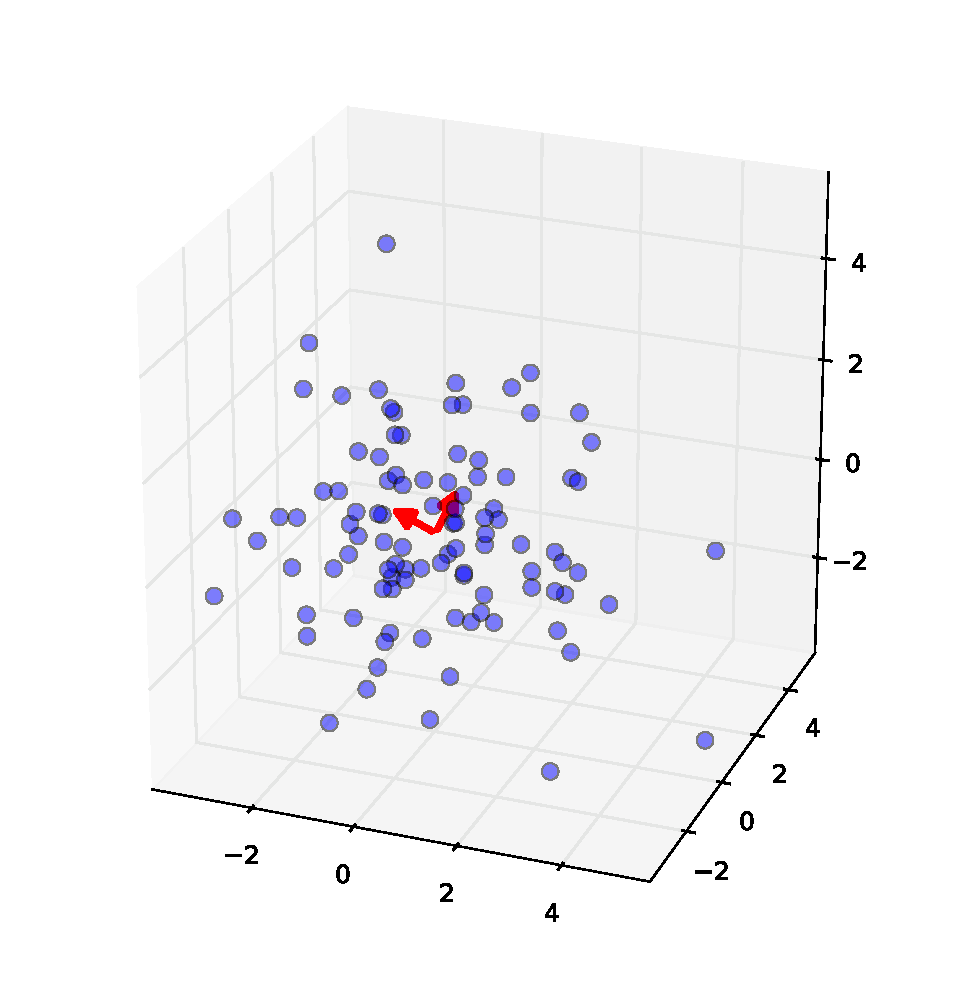
\includegraphics[width=0.5\textwidth]{img/pca/components.pdf}
\end{frame}

\begin{frame}{PCA: projecting and reconstructing (2D)}
\begin{figure}
\begin{tabular}{ccc}
\small{original data} & \small{projection} & \small{reconstruction}\\
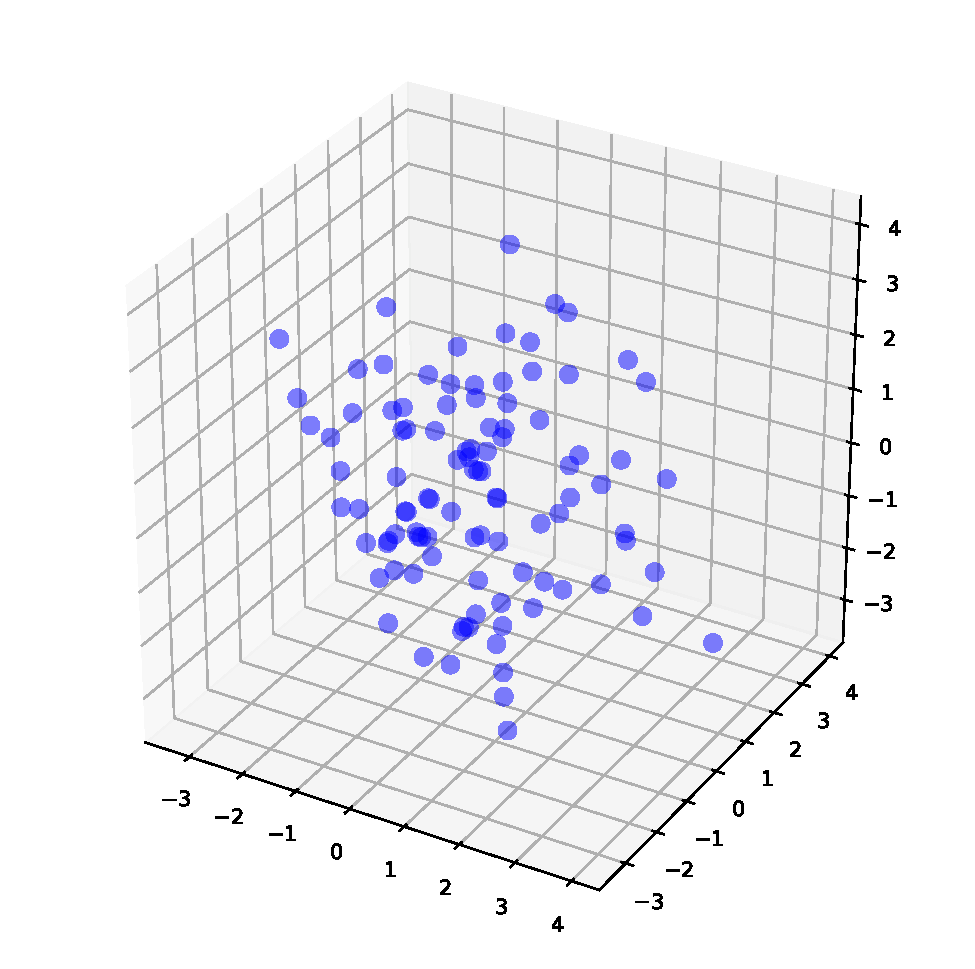
\includegraphics[width=0.3\textwidth]{img/pca/original.pdf}&
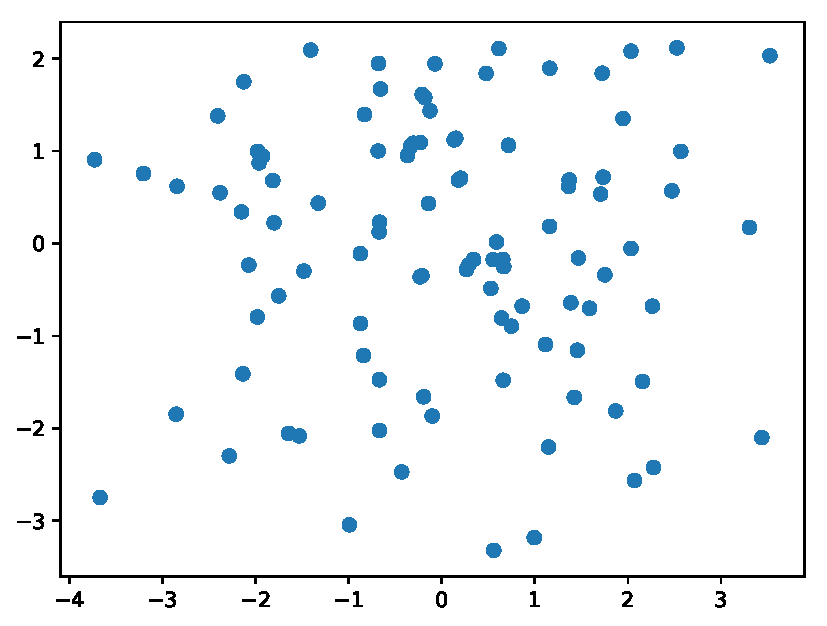
\includegraphics[width=0.3\textwidth]{img/pca/proj.pdf}&
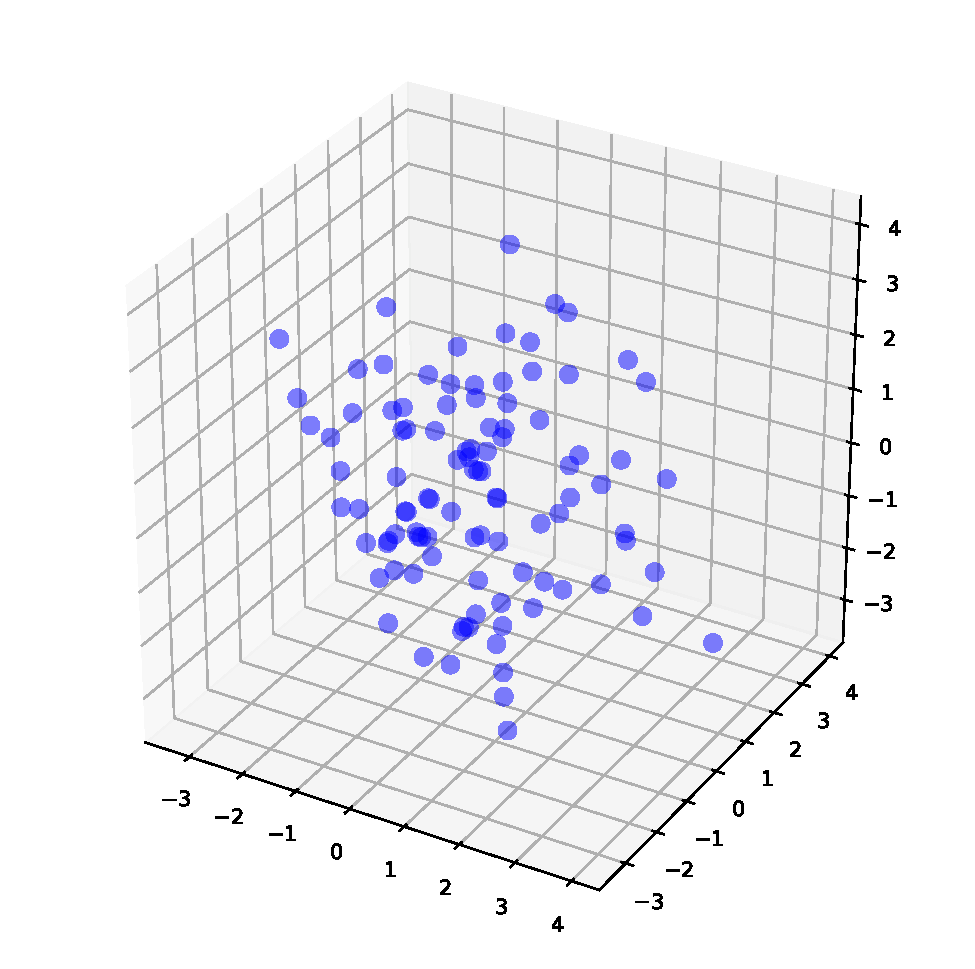
\includegraphics[width=0.3\textwidth]{img/pca/reconstr.pdf}
\end{tabular}
\end{figure}
\end{frame}
\begin{frame}{PCA: projecting and reconstructing (1D)}
\begin{figure}
\begin{tabular}{ccc}
\small{original data} & \small{projection} & \small{reconstruction}\\
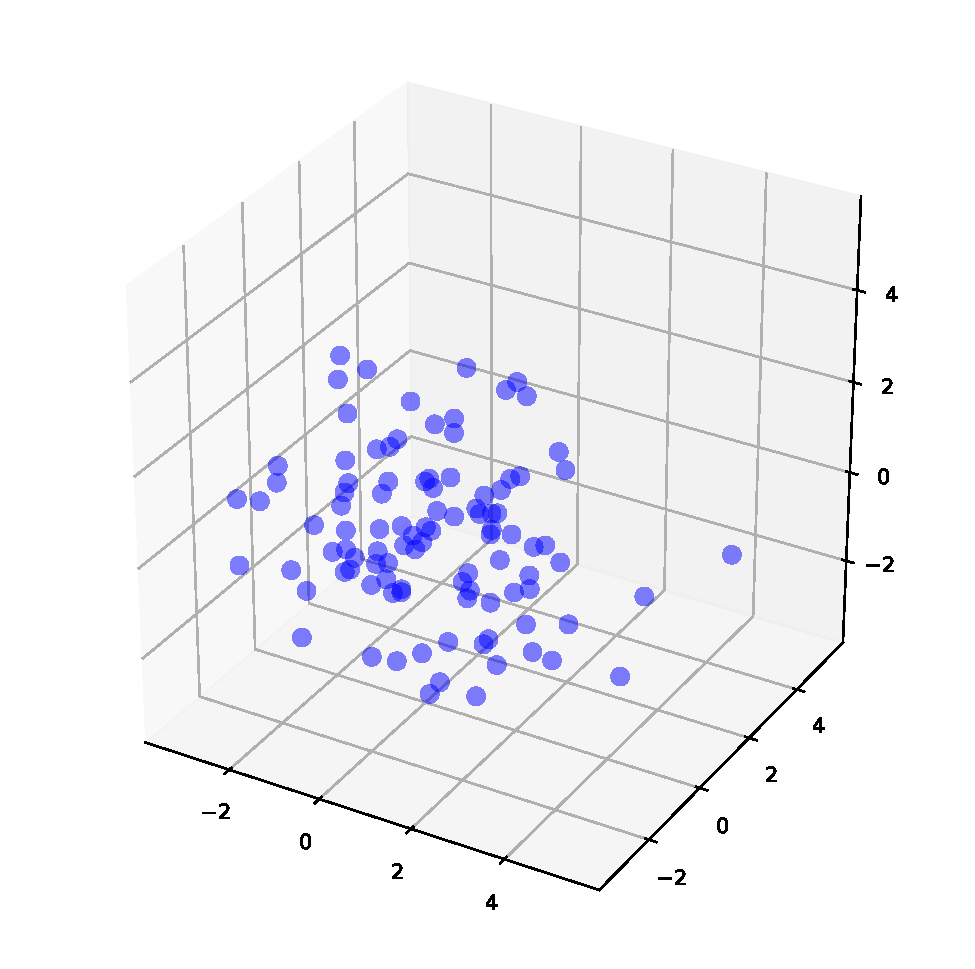
\includegraphics[width=0.3\textwidth]{img/pca/original1.pdf}&
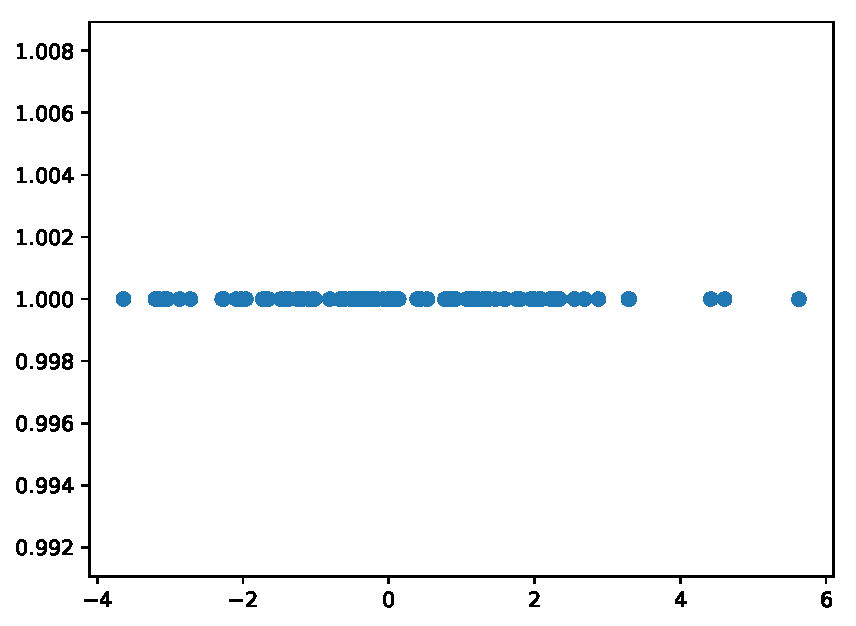
\includegraphics[width=0.3\textwidth]{img/pca/proj1.pdf}&
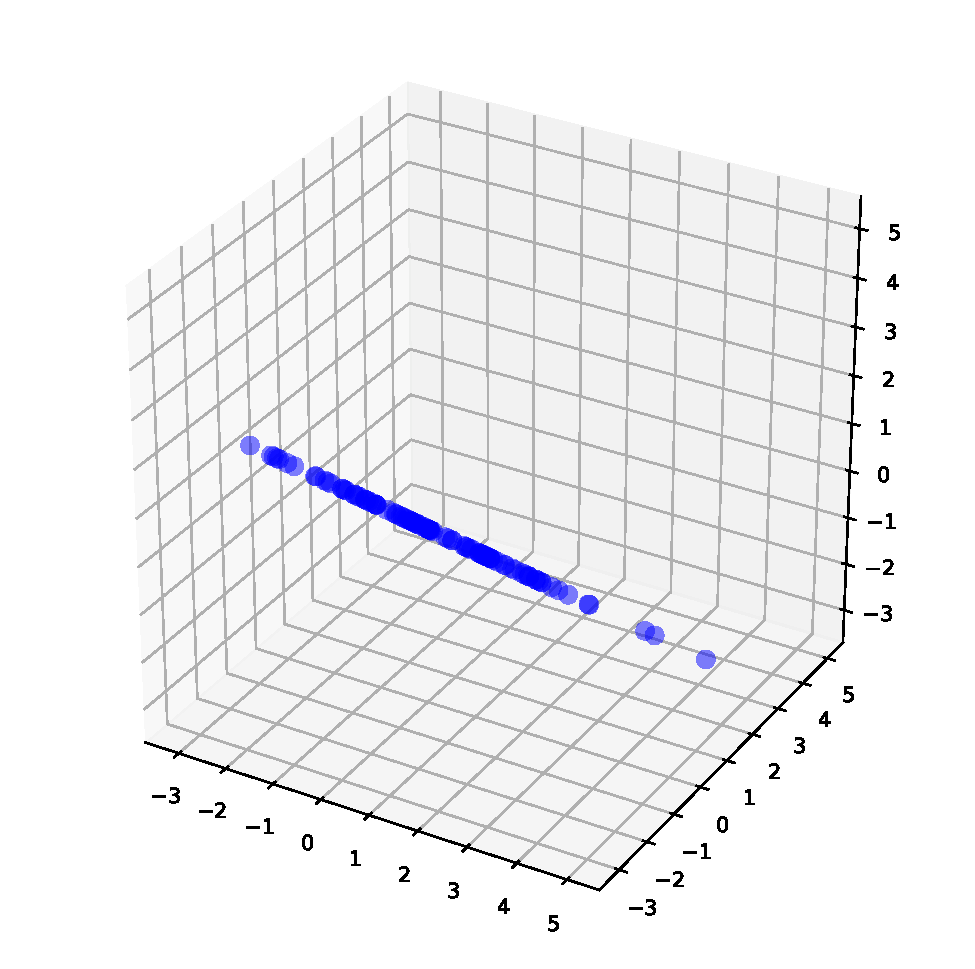
\includegraphics[width=0.3\textwidth]{img/pca/reconstr1.pdf}
\end{tabular}
\end{figure}
\end{frame}

\section{Eigenfaces}
\begin{frame}{Eigenfaces}
Famous algorithm for face recognition. Training is as simple as:
\begin{itemize}
\item load faces and annotations from the Olivetti dataset (datasets.get\_faces\_dataset takes care of loading and flattening images)\\
\begin{center}
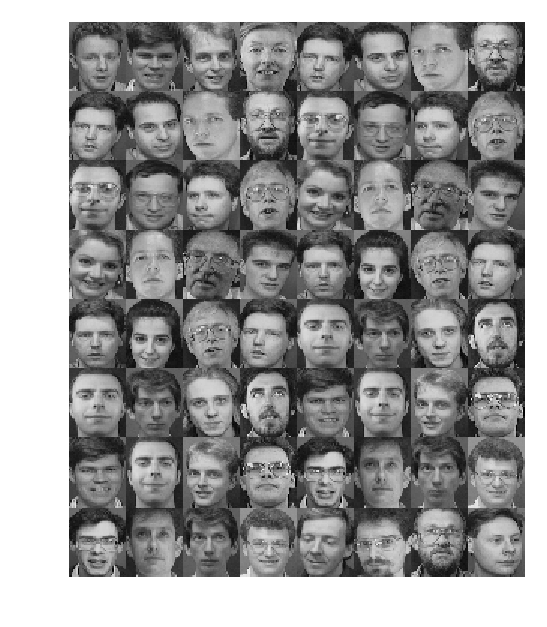
\includegraphics[width=0.2\textwidth]{img/eigenfaces/olivetti.pdf}
\end{center}
\item Select a number of principal components and fit a PCA on training faces 
\end{itemize}
\end{frame}
\begin{frame}{Eigenfaces}
To classify a test image:
\begin{itemize}
\item Project the image in the reduced spaces built in the training phase
\item Perform \textbf{nearest neighbor classification}:
\begin{itemize}
\item Roughly speaking, \underline{choose the class of the nearest training example} (in the reduced space)
\end{itemize}
\end{itemize}
\end{frame}
\begin{frame}{Eigenfaces: a magic trick to compute eigenvectors}
Each Olivetti image is $112\times 92$. Once flattened, is a vector of $10304$ pixels:
\begin{itemize}
\item The convariance matrix is $10304\times 10304$
\item Computing eigenvectors and eigenvalues \underline{is a pain}
\item Instead, compute the covariance matrix of transposed $X$:
\begin{equation*}
\Sigma = (X-\mu)(X-\mu)^T
\end{equation*}
\item Once selected the principal components $\tilde{E}$ of this weirdo space, you can compute the original eigenvectors just like:
\begin{equation*}
E = X^T\cdot \tilde{E}
\end{equation*}
\end{itemize}
\end{frame}
\bgroup
\begin{frame}{Eigenfaces: some plots}
\begin{itemize}
\item Mean face:
\begin{figure}
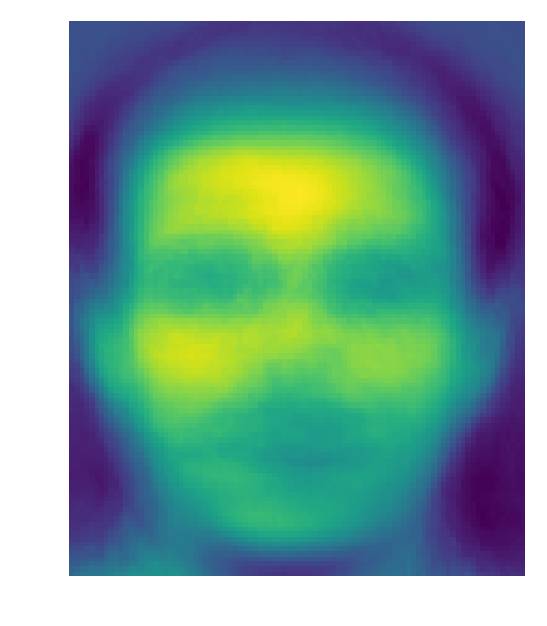
\includegraphics[width=0.18\textwidth]{img/eigenfaces/mean.pdf}
\end{figure}
\item Eigenvectors:
\setlength{\tabcolsep}{.07em}
\begin{figure}
\begin{tabular}{ccccc}
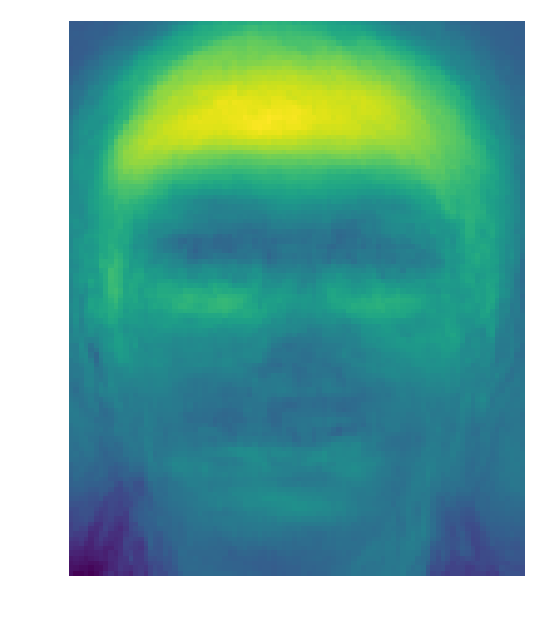
\includegraphics[width=0.18\textwidth]{img/eigenfaces/0.pdf}&
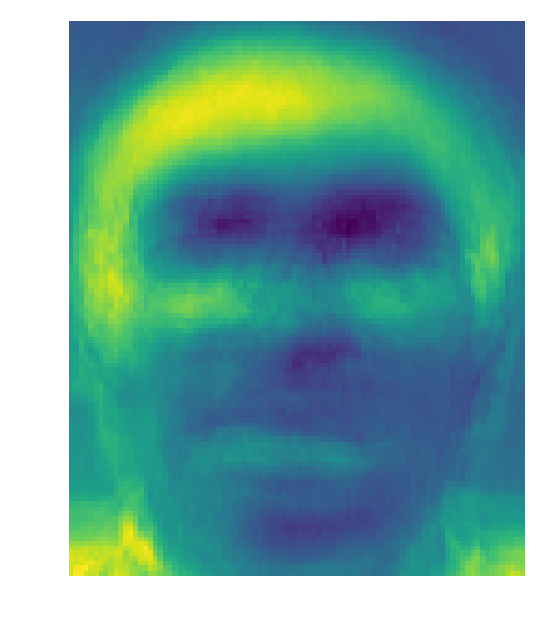
\includegraphics[width=0.18\textwidth]{img/eigenfaces/1.pdf}&
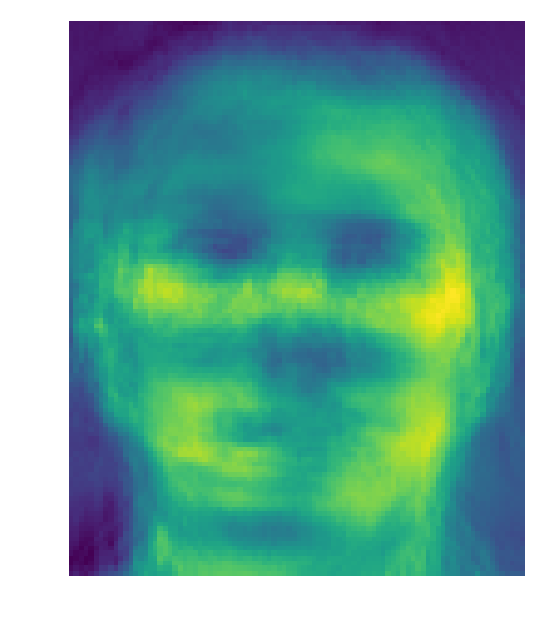
\includegraphics[width=0.18\textwidth]{img/eigenfaces/2.pdf}&
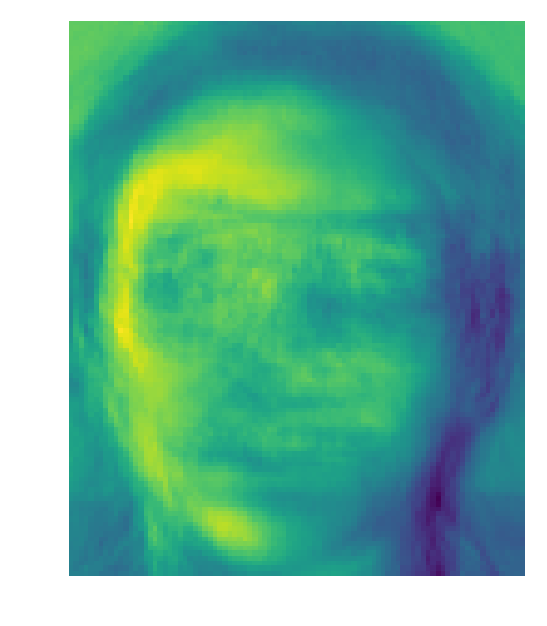
\includegraphics[width=0.18\textwidth]{img/eigenfaces/3.pdf}&
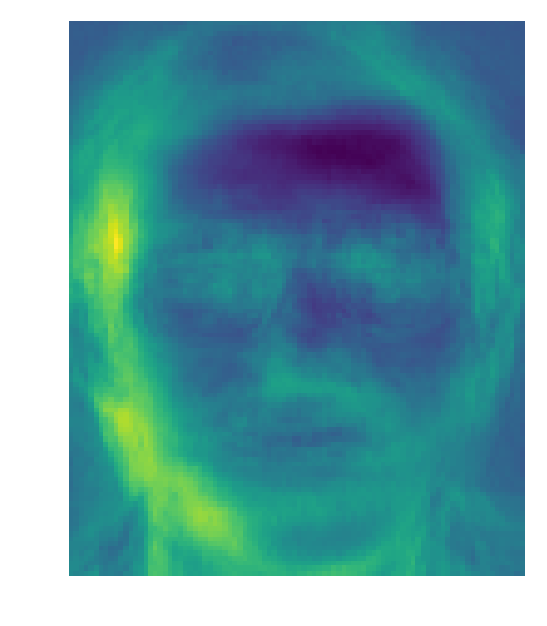
\includegraphics[width=0.18\textwidth]{img/eigenfaces/4.pdf}
\end{tabular}
\end{figure}
\end{itemize}
\end{frame}
\egroup
\begin{frame}{Eigenfaces: face space}
\centering
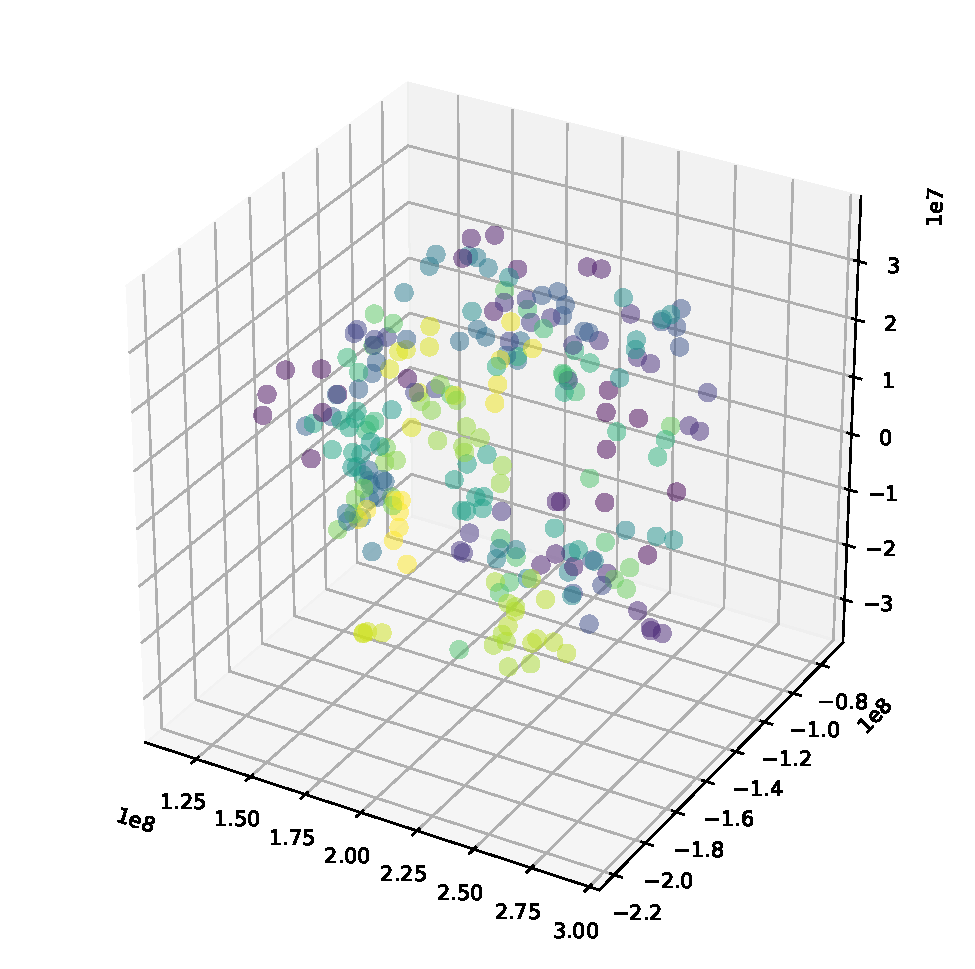
\includegraphics[width=0.5\textwidth]{img/eigenfaces/face_space.pdf}
\end{frame}

\begin{frame}{Eigenfaces: how many dimensions?}
\centering
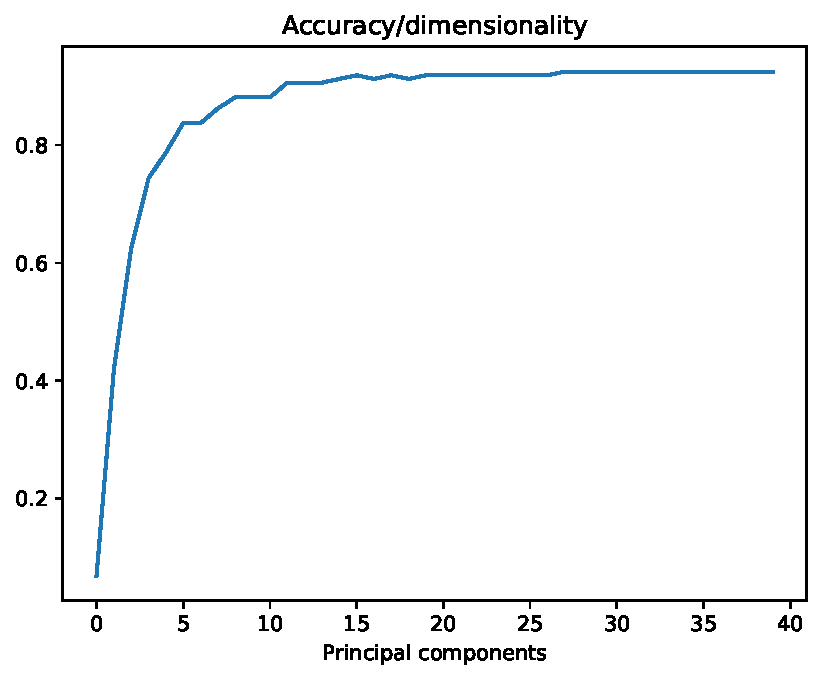
\includegraphics[width=0.5\textwidth]{img/eigenfaces/accuracy.pdf}
\end{frame}



\end{document}